\documentclass[12pt]{article}
\usepackage{graphicx}
\usepackage{amsmath}
\usepackage{float}

\title{Lab 3: Webcam Beam Measurements}
\author{Arnav Menon \\ School of Physics, Georgia Institute of Technology}
\date{February 7, 2025}

\begin{document}

\maketitle

\section{Introduction}
This experiment aimed to measure the transverse intensity profile of a laser beam using a webcam, providing a more comprehensive analysis compared to traditional methods such as the scanning slit and razor blade techniques. While these conventional methods are effective, they are limited to one-dimensional intensity profiles and suffer from resolution constraints. The webcam-based approach enables a full two-dimensional measurement, leveraging software analysis to extract beam properties like divergence and waist.

\section{Procedure}
\subsection{Optical Setup}
The experimental setup was designed to allow for the longest possible beam propagation distance to accurately analyze the beam’s divergence. The laser was installed at one end of the optical table, with optical elements positioned as close as possible to conserve space. The webcam was placed along the beam path, ensuring the beam was centered on the camera sensor and positioned at varying distances to capture the beam's transverse intensity profile.

To prevent sensor saturation, a neutral density (ND) filter was attached to the front of the camera using a lens tube. A filter wheel was used to vary the beam attenuation dynamically.

\subsection{Data Acquisition}
Data collection was conducted using a high-resolution FLIR webcam with a 1440×1080 active pixel array. The camera was interfaced with Igor Pro software for image acquisition and analysis. 

The procedure for capturing images involved:
\begin{itemize}
    \item Launching Igor Pro and opening the ``Exp3'' file to initialize the camera.
    \item Using the ``Camera Operations'' menu to capture single or averaged images (e.g., ``takeone,'' ``take20,'' or ``take200'').
    \item Adjusting the laser power and ND filter settings to ensure an optimal signal-to-noise ratio without sensor saturation.
\end{itemize}

To verify that the camera was not saturated, the maximum recorded pixel value was checked using Igor’s \texttt{WaveMax(mywave)} command. If the maximum value exceeded 4000 (out of a 12-bit range of 4096), attenuation was increased to avoid data clipping. If the signal was below 2000, attenuation was reduced to maximize data quality.

\subsection{Data Processing and Analysis}
After acquiring the beam images, the intensity distribution was analyzed using Igor Pro. The following steps were performed:
\begin{enumerate}
    \item Image scaling was defined based on the pixel size (3.45 um per pixel), using Igor’s SetScale function.
    \item The grayscale beam image was visualized, and a two-dimensional Gaussian fit was applied using the Igor Curve Fitting tool.
    \item The fitted parameters were extracted, including beam waist, orientation, and background noise level.
    \item The Gaussian fit was refined to improve accuracy by generating a high-resolution fit.
\end{enumerate}

The beam width was measured at multiple distances from the laser to determine its divergence. The camera was moved incrementally along the beam path, with measurements recorded approximately every 50 mm. At each position:
\begin{itemize}
    \item The beam width was measured in both horizontal and vertical directions.
    \item A Gaussian fit was applied to extract the waist parameters.
    \item The distance from the laser source was carefully measured and recorded.
\end{itemize}

\subsection{Beam Divergence Measurement}
To analyze the beam’s divergence, the beam width was plotted as a function of distance from the laser. The data was fitted to a linear model for large distances (\textgreater 500 mm) and compared to the theoretical Gaussian beam propagation equation:

\begin{equation}
    w(z) = w_0 \sqrt{1 + \left( \frac{z}{z_R} \right)^2 }
\end{equation}

where \( w_0 \) is the beam waist and \( z_R \) is the Rayleigh range, given by:

\begin{equation}
    z_R = \frac{\pi w_0^2}{\lambda}
\end{equation}

with \( \lambda = 633 \) nm for the HeNe laser used in this experiment. The fitted waist size was compared to theoretical expectations. These results were used to evaluate the effectiveness of webcam-based beam profiling and compare it to traditional slit and razor blade measurement techniques.

\section{Results}
\subsection{Beam Profile}
The captured beam profile image is shown in Figure \ref{fig:beam_profile}. The image highlights the Gaussian nature of the beam intensity distribution.

\begin{figure} [H]
    \centering
    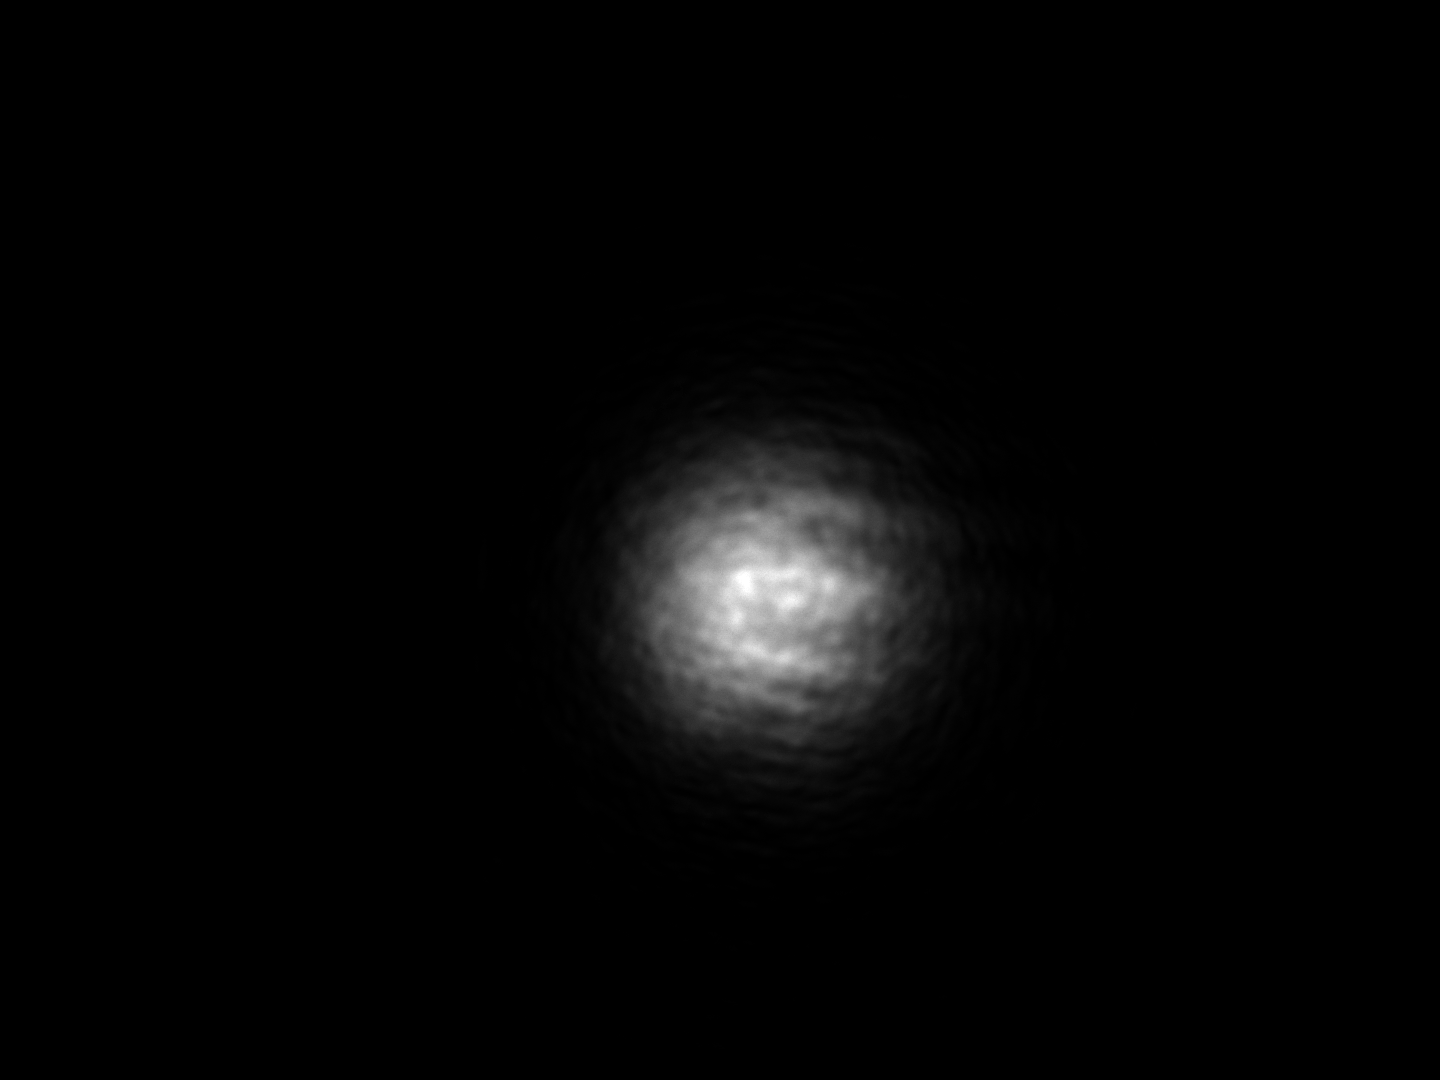
\includegraphics[width=0.6\textwidth]{Lab Modern Optics Image.png}
    \caption{Captured beam profile image. The maximum value was checked to ensure that the image is not oversaturated.}
    \label{fig:beam_profile}
\end{figure}

\subsection{Beam Divergence}
The horizontal and vertical beam widths were measured at multiple distances, and the results are plotted in Figure \ref{fig:beam_divergence}. These measurements illustrate the beam’s divergence characteristics. There is a gap in the measurements between 1 meter and 1.5 meters due to the size of the breadboard and mirror setup used in the experiment.

\begin{figure} [H]
    \centering
    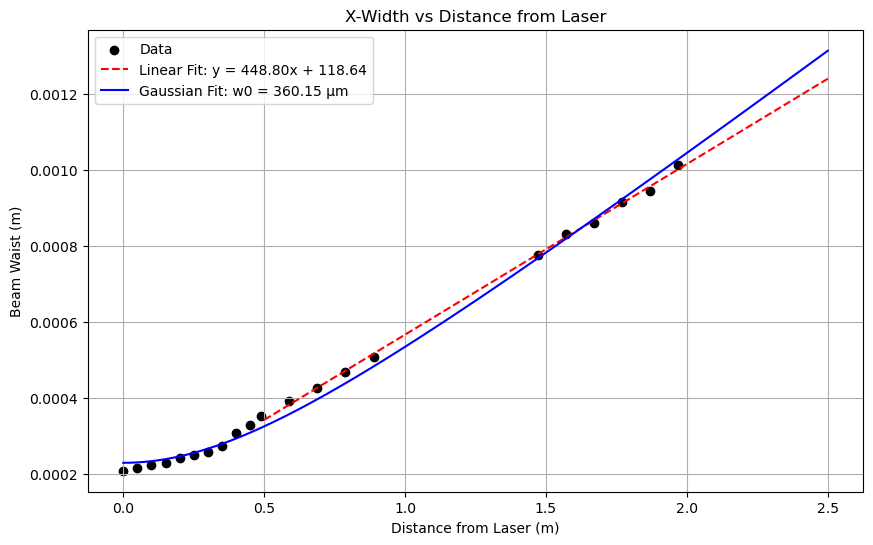
\includegraphics[width=0.8\textwidth]{o1.png}
    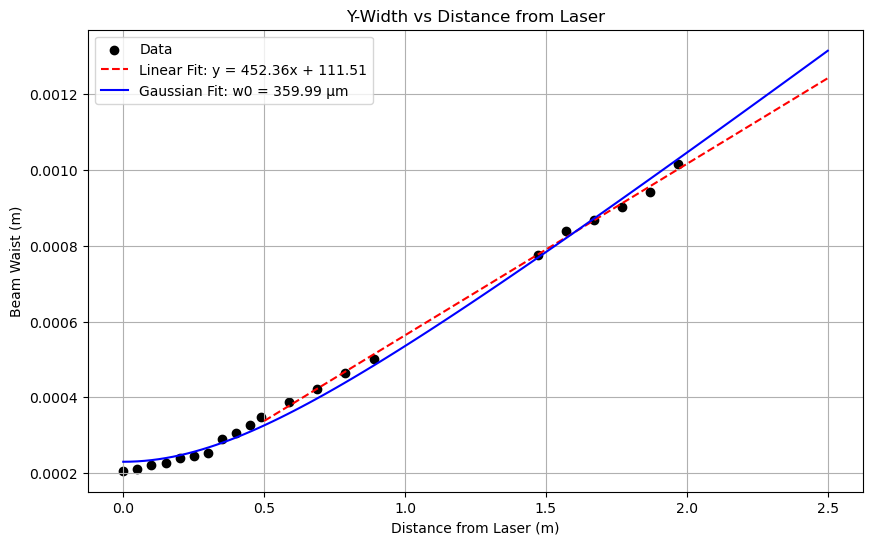
\includegraphics[width=0.8\textwidth]{o2.png}
    \caption{Beam width as a function of distance from the laser source. The dashed red lines indicate the linear fit to the far measurements, and the blue solid line shows the Gaussian fit to the entire data. The graphs show a clear distinction between the near and far measurements. }
    \label{fig:beam_divergence}
\end{figure}

A three-dimensional visualization of the beam intensity profile, generated using Igor's Gizmo tool, is shown in Figure \ref{fig:3d_beam}. This representation provides an intuitive view of the intensity distribution.

\begin{figure} [H]
    \centering
    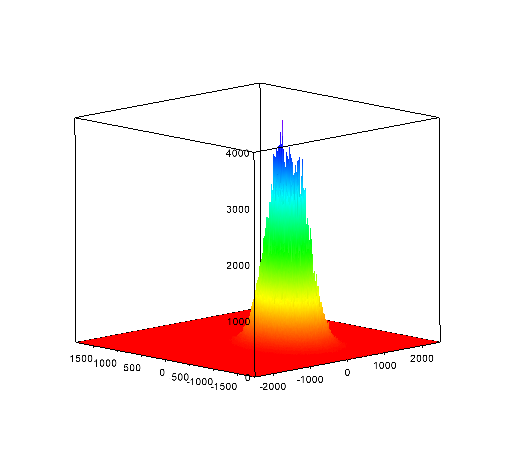
\includegraphics[width=0.6\textwidth]{Lab 3 Gizmo.png}
    \caption{3D representation of the beam profile.}
    \label{fig:3d_beam}
\end{figure}

\section{Conclusion}
The webcam-based beam profile measurements were consistent with theoretical Gaussian beam predictions. The results aligned well with expected divergence trends, demonstrating the method’s effectiveness. Compared to traditional techniques, the webcam approach offered a more detailed and efficient way to analyze beam properties, reducing manual effort and increasing spatial resolution. This experiment successfully demonstrated the use of a webcam for laser beam profiling. The method provided accurate, high-resolution measurements of the beam waist and divergence. Future improvements could include automating data acquisition and refining the fitting algorithms for increased precision.

\end{document}


